\section{Data Analysis and Computations}
\label{sec:analysis}

\subsection{Preprocessing}

Each observation's six-feature representation (Section~\ref{sec:methodology})
is built \emph{pointwise}: every feature except $\Delta t$ is a function of
that single observation's own (flux, flux\_err, $\lambda_\mathrm{eff}$,
is\_detection) fields alone, with no running statistic computed over the
object's other observations. Concretely, the flux features are
$\mathrm{signed\_log1p}(\mathrm{flux}/\mathrm{flux\_err})$,
$\mathrm{signed\_log1p}(\mathrm{flux})$, and $\log1p(\mathrm{flux\_err})$,
where $\mathrm{signed\_log1p}(x) \equiv \mathrm{sign}(x)\log1p(|x|)$. This
choice is deliberate and leakage-free by construction, for two independent
reasons. First, $\mathrm{flux\_err} > 0$ is a per-observation schema
invariant, true for every observation regardless of any other observation,
so the ratio $\mathrm{flux}/\mathrm{flux\_err}$ never requires an epsilon
floor or a survey-specific clipping constant to stay finite -- it is simply
signal-to-noise, well defined on a single point. Second, because no feature
depends on anything computed over a window of the light curve, there is no
running statistic that must be kept synchronised between offline batch
tensorisation (iterating an archived Parquet file) and streaming inference
(updating state one Kafka message at a time); an off-by-one in ``does the
running maximum include the current point'' is a live-only bug class this
scheme cannot exhibit, since it has no running state to get wrong in the
first place.

\subsection{Windowing}
\label{sec:windowing}

The training corpus's archived SNANA dump gives each object its
\emph{complete} simulated observation history, including entire observing
seasons before the transient ever explodes. A live alert, by contrast,
carries only detections to date plus forced photometry reaching back a
bounded window before the object's first detection. These are structurally
different artifacts, not merely different volumes of the same thing:
training on the former means training on an input distribution a live
system will never actually present at inference time.

Measured directly on a class-stratified \WindowNSampleObjects{}-object sample of Tier A (reconstructed from the interim parquet via the same reader
and tensorisation code used in production), the unwindowed mean is
\WindowMeanDetections{} detections against \WindowMeanForcedPhot{} forced-
photometry points per object -- the training corpus is, on average, about
\WindowForcedToDetRatio{} times longer than what a live stream would ever accumulate
for the same object. Applying the pipeline's 30-day pre-detection lookback
window reduces the mean sequence length from \WindowMeanSeqLenUnwindowed{}
to \WindowMeanSeqLenWindowed{} observations, a \WindowFracRemoved{}\%
reduction (Figure~\ref{fig:windowhist}).

\begin{figure}[htb]
\centering
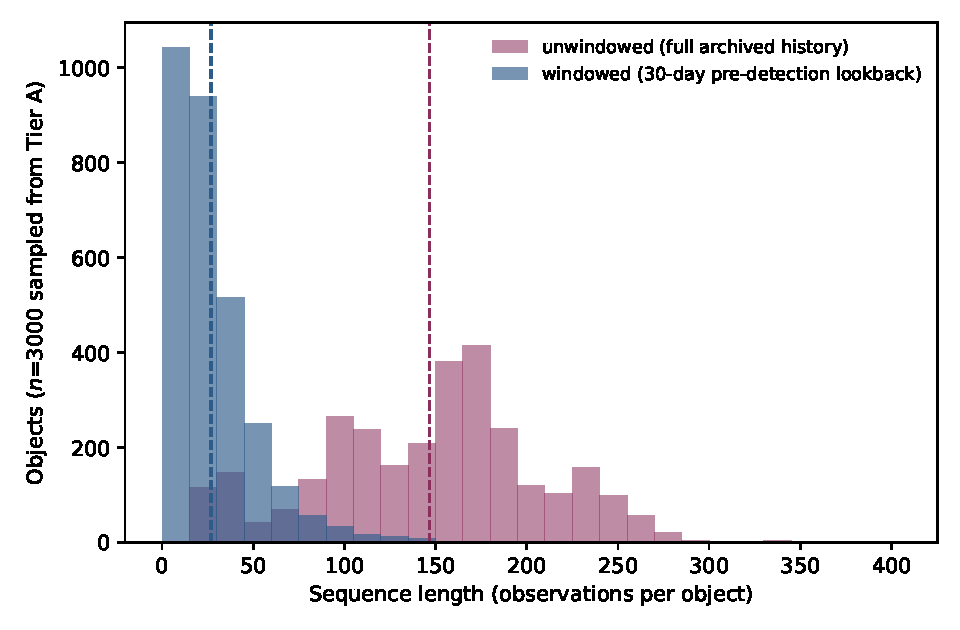
\includegraphics[width=0.72\linewidth]{figures/fig3_windowing_histograms}
\caption{Per-object sequence length, unwindowed (full archived history)
versus windowed (30-day pre-detection lookback), for the same
\WindowNSampleObjects{}-object stratified Tier A sample. Dashed lines mark
each distribution's mean. Windowing does not merely shorten sequences
uniformly; it collapses the distribution onto the much shorter range a
live alert stream actually produces.}
\label{fig:windowhist}
\end{figure}

This left-edge window bounds only how far back a sequence may reach. It
does not bound how far \emph{forward} a sequence may extend, and for a
fading transient this rarely matters -- the object drops below the
detection threshold and its own last detection arrives naturally soon after
its first. For a recurring or continuously variable source, nothing fades,
so a sequence's right edge sits wherever the underlying simulation happened
to end, independent of anything resembling a supernova's characteristic
timescale. Table~\ref{tab:spans} reports this directly, computed from the
raw ELAsTiCC2 exotic-class model directories: a tidal disruption event
(TDE, a bounded, fading transient) has a mean detection span of
\ExoticSpanMeanTDE{} days, while an eclipsing binary (EB) and a changing-look
AGN (CLAGN) -- both continuously variable, non-fading sources -- have mean
spans of \ExoticSpanMeanEB{} and \ExoticSpanMeanCLAGN{} days respectively,
\ExoticSpanRatioEB{}--\ExoticSpanRatioCLAGN{}$\times$ longer, despite a per-object observation count only
\ExoticNobsMeanEB{}--\ExoticNobsMeanCLAGN{} versus TDE's \ExoticNobsMeanTDE{}
(about \ExoticNobsRatioEB{}--\ExoticNobsRatioCLAGN{}$\times$, not \ExoticSpanRatioEB{}--\ExoticSpanRatioCLAGN{}$\times$). The right edge is therefore
unbounded in practice for exactly the class of object a live serving system
will keep re-observing indefinitely.

\begin{table}[htb]
\centering
\caption{Mean/median detection span and mean observation count per object,
computed directly from the raw ELAsTiCC2 model directories for one fading
transient (TDE) and two continuously-variable, non-fading sources (EB,
CLAGN). Detection span is $\max{-}\min$ of an object's own detection-flagged
observation times; all three directories were read in full with zero
discarded objects.}
\label{tab:spans}
\begin{tabular}{lrrrr}
\toprule
Class & $N$ objects & Mean span (d) & Median span (d) & Mean NOBS \\
\midrule
TDE (fading) & \ExoticNObjectsTDE{} & \ExoticSpanMeanTDE{} &
  \ExoticSpanMedianTDE{} & \ExoticNobsMeanTDE{} \\
EB (non-fading) & \ExoticNObjectsEB{} & \ExoticSpanMeanEB{} &
  \ExoticSpanMedianEB{} & \ExoticNobsMeanEB{} \\
CLAGN (non-fading) & \ExoticNObjectsCLAGN{} & \ExoticSpanMeanCLAGN{} &
  \ExoticSpanMedianCLAGN{} & \ExoticNobsMeanCLAGN{} \\
\bottomrule
\end{tabular}
\end{table}

A right-edge cap, \texttt{max\_span\_days}, was added and ablated at
$\{100, 200, \text{uncapped}\}$ days, evaluated by inference only against
the already-trained Tier A checkpoint (Table~\ref{tab:spanablation}).
\SpanChosenDefault{} days gives the best full-cutoff macro-F1 among the two finite settings
tested, costs only \SpanTwoHundredCost{} macro-F1 relative to uncapped, and
truncates at most \SpanTwoHundredMaxAffected{}\% of any class's objects. This value, \SpanChosenDefault{} days, was
adopted as the default the serving path passes explicitly; the underlying
function's own parameter default is left unchanged (\texttt{None}, i.e.\
uncapped) so that no existing training or evaluation call site is affected
by the change. Capping CLAGN's window at \SpanChosenDefault{} days more than triples its
mean classifier entropy (from \ClagnEntropyUncapped{} to
\ClagnEntropyCapped{}) and pulls its mean maximum softmax probability down
from \ClagnMaxProbUncapped{} to \ClagnMaxProbCapped{}, on the same
\ClagnNObjects{}-object population -- a real, measurable step toward
appropriate uncertainty on an out-of-distribution input, though still short
of a genuinely in-distribution object's own baseline confidence
(Section~\ref{sec:discussion}).

\begin{table}[htb]
\centering
\caption{Right-edge span ablation, Tier A test set, full cutoff, inference
only against the existing trained checkpoint (no retraining under any
cap).}
\label{tab:spanablation}
\begin{tabular}{lrrrr}
\toprule
\texttt{max\_span\_days} & Macro-F1 & Ia affected & Ib/c affected & II affected \\
\midrule
100 & \SpanHundredMacroF{} & \SpanHundredAffectedIa{}\% & \SpanHundredAffectedIbc{}\% & \SpanHundredAffectedII{}\% \\
\textbf{200 (chosen)} & \SpanTwoHundredMacroF{} & \SpanTwoHundredAffectedIa{}\% & \SpanTwoHundredAffectedIbc{}\% & \SpanTwoHundredAffectedII{}\% \\
Uncapped & \SpanUncappedMacroF{} & 0\% & 0\% & 0\% \\
\bottomrule
\end{tabular}
\end{table}

\subsection{Flux calibration}

Every reader in this pipeline is responsible for converting its source's
native photometric convention onto one shared scale before a canonical
alert is ever constructed: the SNANA \texttt{FLUXCAL} convention, AB
zeropoint 27.5. ELAsTiCC2's simulated flux already sits on this zeropoint,
so its reader performs no conversion at all -- an exception specific to
that one source, not a template for any other reader. A real ZTF alert
instead carries a PSF-fit magnitude and uncertainty
(\texttt{magpsf}/\texttt{sigmapsf}) referenced against that \emph{specific
alert's own} photometric zeropoint, \texttt{magzpsci}, which was measured
to vary row to row (across the full Tier B corpus, and again independently
on one live-polled Fink alert packet). Treating \texttt{magzpsci} as a
fixed constant, rather than reading it per row, would introduce a
brightness-dependent calibration error rather than a uniform shift -- worst
in exactly the faint, early-time regime this pipeline is built to classify
early. The conversion is
\begin{align}
  \mathrm{flux}_\mathrm{raw} &= \mathrm{sign} \times 10^{-0.4(\mathrm{magpsf} - \mathrm{magzpsci})}, \\
  \mathrm{flux\_err}_\mathrm{raw} &= |\mathrm{flux}_\mathrm{raw}| \times \frac{\ln 10}{2.5} \times \mathrm{sigmapsf},
\end{align}
followed by a rescaling from \texttt{magzpsci} onto \texttt{FLUXCAL}
zeropoint 27.5, applied per row through one shared, tested helper every
non-SNANA reader calls:
\begin{equation}
  \mathrm{flux}_{27.5} = \mathrm{flux}_\mathrm{zp} \times 10^{(27.5 - \mathrm{zp})/2.5},
\end{equation}
the only direction that leaves $\mathrm{mag} = \mathrm{zp} - 2.5\log_{10}\mathrm{flux}$
unchanged; LSST's nanojansky fluxes (zeropoint 31.4) are rescaled the same
way. The signal-to-noise feature ($\mathrm{flux}/\mathrm{flux\_err}$) is
scale-invariant and survives a calibration bug of this kind unchanged,
since the erroneous zeropoint factor cancels in the ratio; the
absolute-flux feature does not, and carries a silent, brightness-dependent
distortion into training with no symptom that looks like an error. This
is not hypothetical: an earlier version of the helper applied the
reciprocal factor, and Section~\ref{sec:silentfailures} describes what it
did and how it was found.

\subsection{Training protocol}

Splits are assigned by object identifier (checked for duplicates), never by
observation, so no object's light curve is divided across splits. Tier A
training uses class-weighted cross-entropy (sqrt-dampened inverse-class-
frequency weights, applied mildly rather than fully rebalancing toward the
real sky rate -- Section~\ref{sec:discussion}), AdamW, and cosine-annealed
learning-rate decay (Appendix~\ref{sec:appendixa} gives every hyperparameter
in full). The Tier B fine-tune uses a two-phase, discriminative
learning-rate schedule: the GRU trunk is frozen for the first two epochs
(only the head, and, where present, the static branch, train, at a
comparatively high learning rate), then unfrozen for six further epochs at
a learning rate $100\times$ lower than the head's own. This asymmetry is
deliberate: the Tier A encoder is the only part of this model that has ever
seen a negative-flux input (Tier B is \TierBNegFluxFrac{}\% negative-flux by construction,
Section~\ref{sec:discussion}), and Tier B's small, positive-flux-only
training set must be allowed to adapt the model to real ZTF cadence and
noise characteristics without being allowed to overwrite what the trunk
already learned about an input regime Tier B cannot itself supply, but
which live Tier C traffic already has.

\subsection{Metrics}

Accuracy is not used as a reportable metric anywhere in this report: on
this project's own class balance (and more strongly on the real sky rate),
a classifier that always predicts the majority class scores well on
accuracy while carrying no useful information at all. Macro-F1 -- the
unweighted mean of each class's own F1 score -- is used instead throughout,
since it cannot be inflated by favouring the common class over the rare
one. Per-class precision, recall, PR-AUC, ROC-AUC, and expected calibration
error are reported alongside macro-F1 for a fuller per-class picture
(Section~\ref{sec:results}). Because this is fundamentally an
\emph{early}-classification problem (Section~\ref{sec:introduction}), the
primary reported figure throughout is macro-F1 as a function of days since
an object's own first detection (the ``phase cutoff''), not a single
end-of-light-curve number: a model that only performs well once a light
curve has fully played out is of limited use to a system whose entire
purpose is to flag an object for spectroscopic follow-up \emph{while} it is
still interesting.
